\chapter{Проведение эксперимента и обработка результатов}

\section{Постановка эксперимента}

\subsection{Конфигурация экспериментального стенда}

\subsubsection{Аппаратное обеспечение}

Процессор Intel(R) Xeon(R) Platinum 8168 CPU 2.7 GHz.
Технология Hyper-Threading отключена для уменьшения влияния на время обработки заявок в системе \cite{LowLatencyHT}.

Оперативная память: DDR4-2666 128 GiB.

\subsubsection{Программное обеспечение}

Операционная система Red Hat Enterprise Linux Server release 7.8 (Maipo).
Ядро Linux 3.10.0-1127.el7.x86\_64

Компилятор C++ Clang 6.0.1.

Стандартная библиотека C++: libstdc++ 8.1.0.

Библиотека Boost.Interprocess 1.68.0.

\subsection{Конфигурация экспериментальной системы}

Система для проведения эксперимента состоит из двух процессов:
\begin{itemize}
\item Процесс-шлюз отвечает за преобразование заявок из формата внешнего мира во внутренний формат системы и обратно. 
\item Процесс-обработчик совершает некоторые преобразования над заявкой и отправляет результат за пределы системы через процесс-шлюз.
\end{itemize}

Процессы выполняются на двух процессорах, расположенных в разных разъемах на материнской плате физического узла.

Снаружи системы находится симулятор внешнего мира. Он генерирует поток заявок в систему и получает результат обработки заявки в системе. Схема взаимодействия процессов в эксперименте представлена на Рисунке \ref{chapter41:SystemSchema}.

\begin{figure}[!h]
\caption{Схема взаимодействия процессов в эксперименте}
\label{chapter41:SystemSchema}
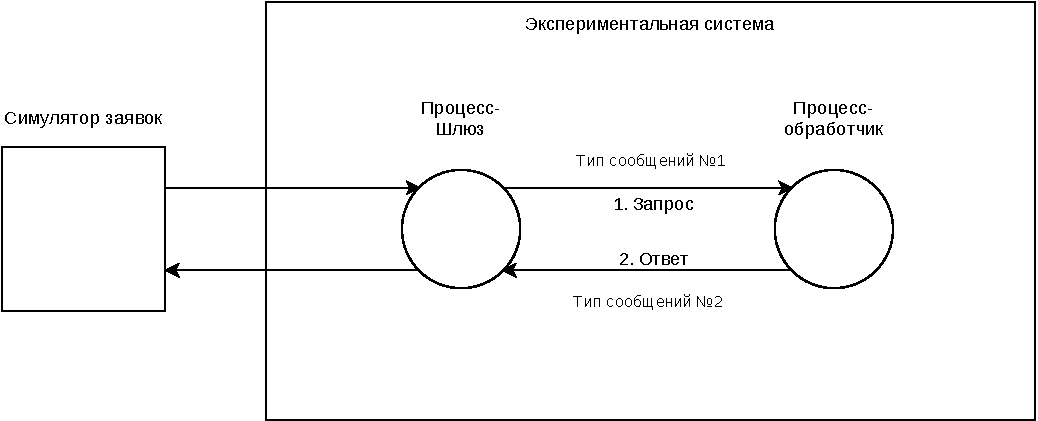
\includegraphics[width=\textwidth]{../../graphics/schemes/SystemSchema}
\end{figure}

В настоящей работе замеряется временная задержка на передачу данных между процессами внутри системы, а именно из процесса-шлюза в процесс-обработчик и обратно (сообщения типа №1 и №2 в запросе и ответе между процессом-шлюзом и процессом обработчиком на Рисунке \ref{chapter41:SystemSchema}).

\subsection{Характер экспериментальной нагрузки}

\textbf{TBD: может, стоит пояснить, почему вместо 5мс получился такой разброс между сериями?}
Симулятор заявок каждые \textit{10 $\pm$ 4 мс} создает и отправляет \textit{4} заявки с интервалом \textit{50 $\pm$ 26 мкс} между ними. Интервалы указаны с 95\% доверительной вероятностью. 

\textbf{TBD: Подозрительный текст. Может, убрать пункт про варьирование размера сообщений типа №1}
Размер сообщений типа №1 (см. Рисунок \ref{chapter41:SystemSchema}) выбирается в зависимости от приходящих в процесс-шлюз заявок с равной вероятностью между 85, 96 и 104 байтами. Размер сообщений типа №2 равен 530 байтам.

\textbf{TBD: тоже стоит убрать. На моих гистограммах этого не видно. Нужны гораздо более искуственные замеры, чтобы обнаружить разницу.}
Различие в размерах сообщений, передаваемых между процессами, позволяет количественно оценить влияние непосредственно размера сообщения на временную задержку на его передачу.

\subsection{Время обслуживания заявок в процессах}
\textbf{TBD: разобраться с обработкой соединений и обслуживанием заявок. Должно быть одно слово для обозначения одной сущности.}

На Рисунке \ref{chapter41:EngineLatency} представлена гистограмма времени обслуживания заявок в процессе-обработчике. Время обслуживания заявок с 95\% доверительной вероятностью укладывается в диапазон \textit{12 $\pm$ 6 мкс}.
\begin{figure}[!h]
\caption{Гистограмма времени обслуживания заявки в процессе-обработчике}
\label{chapter41:EngineLatency}
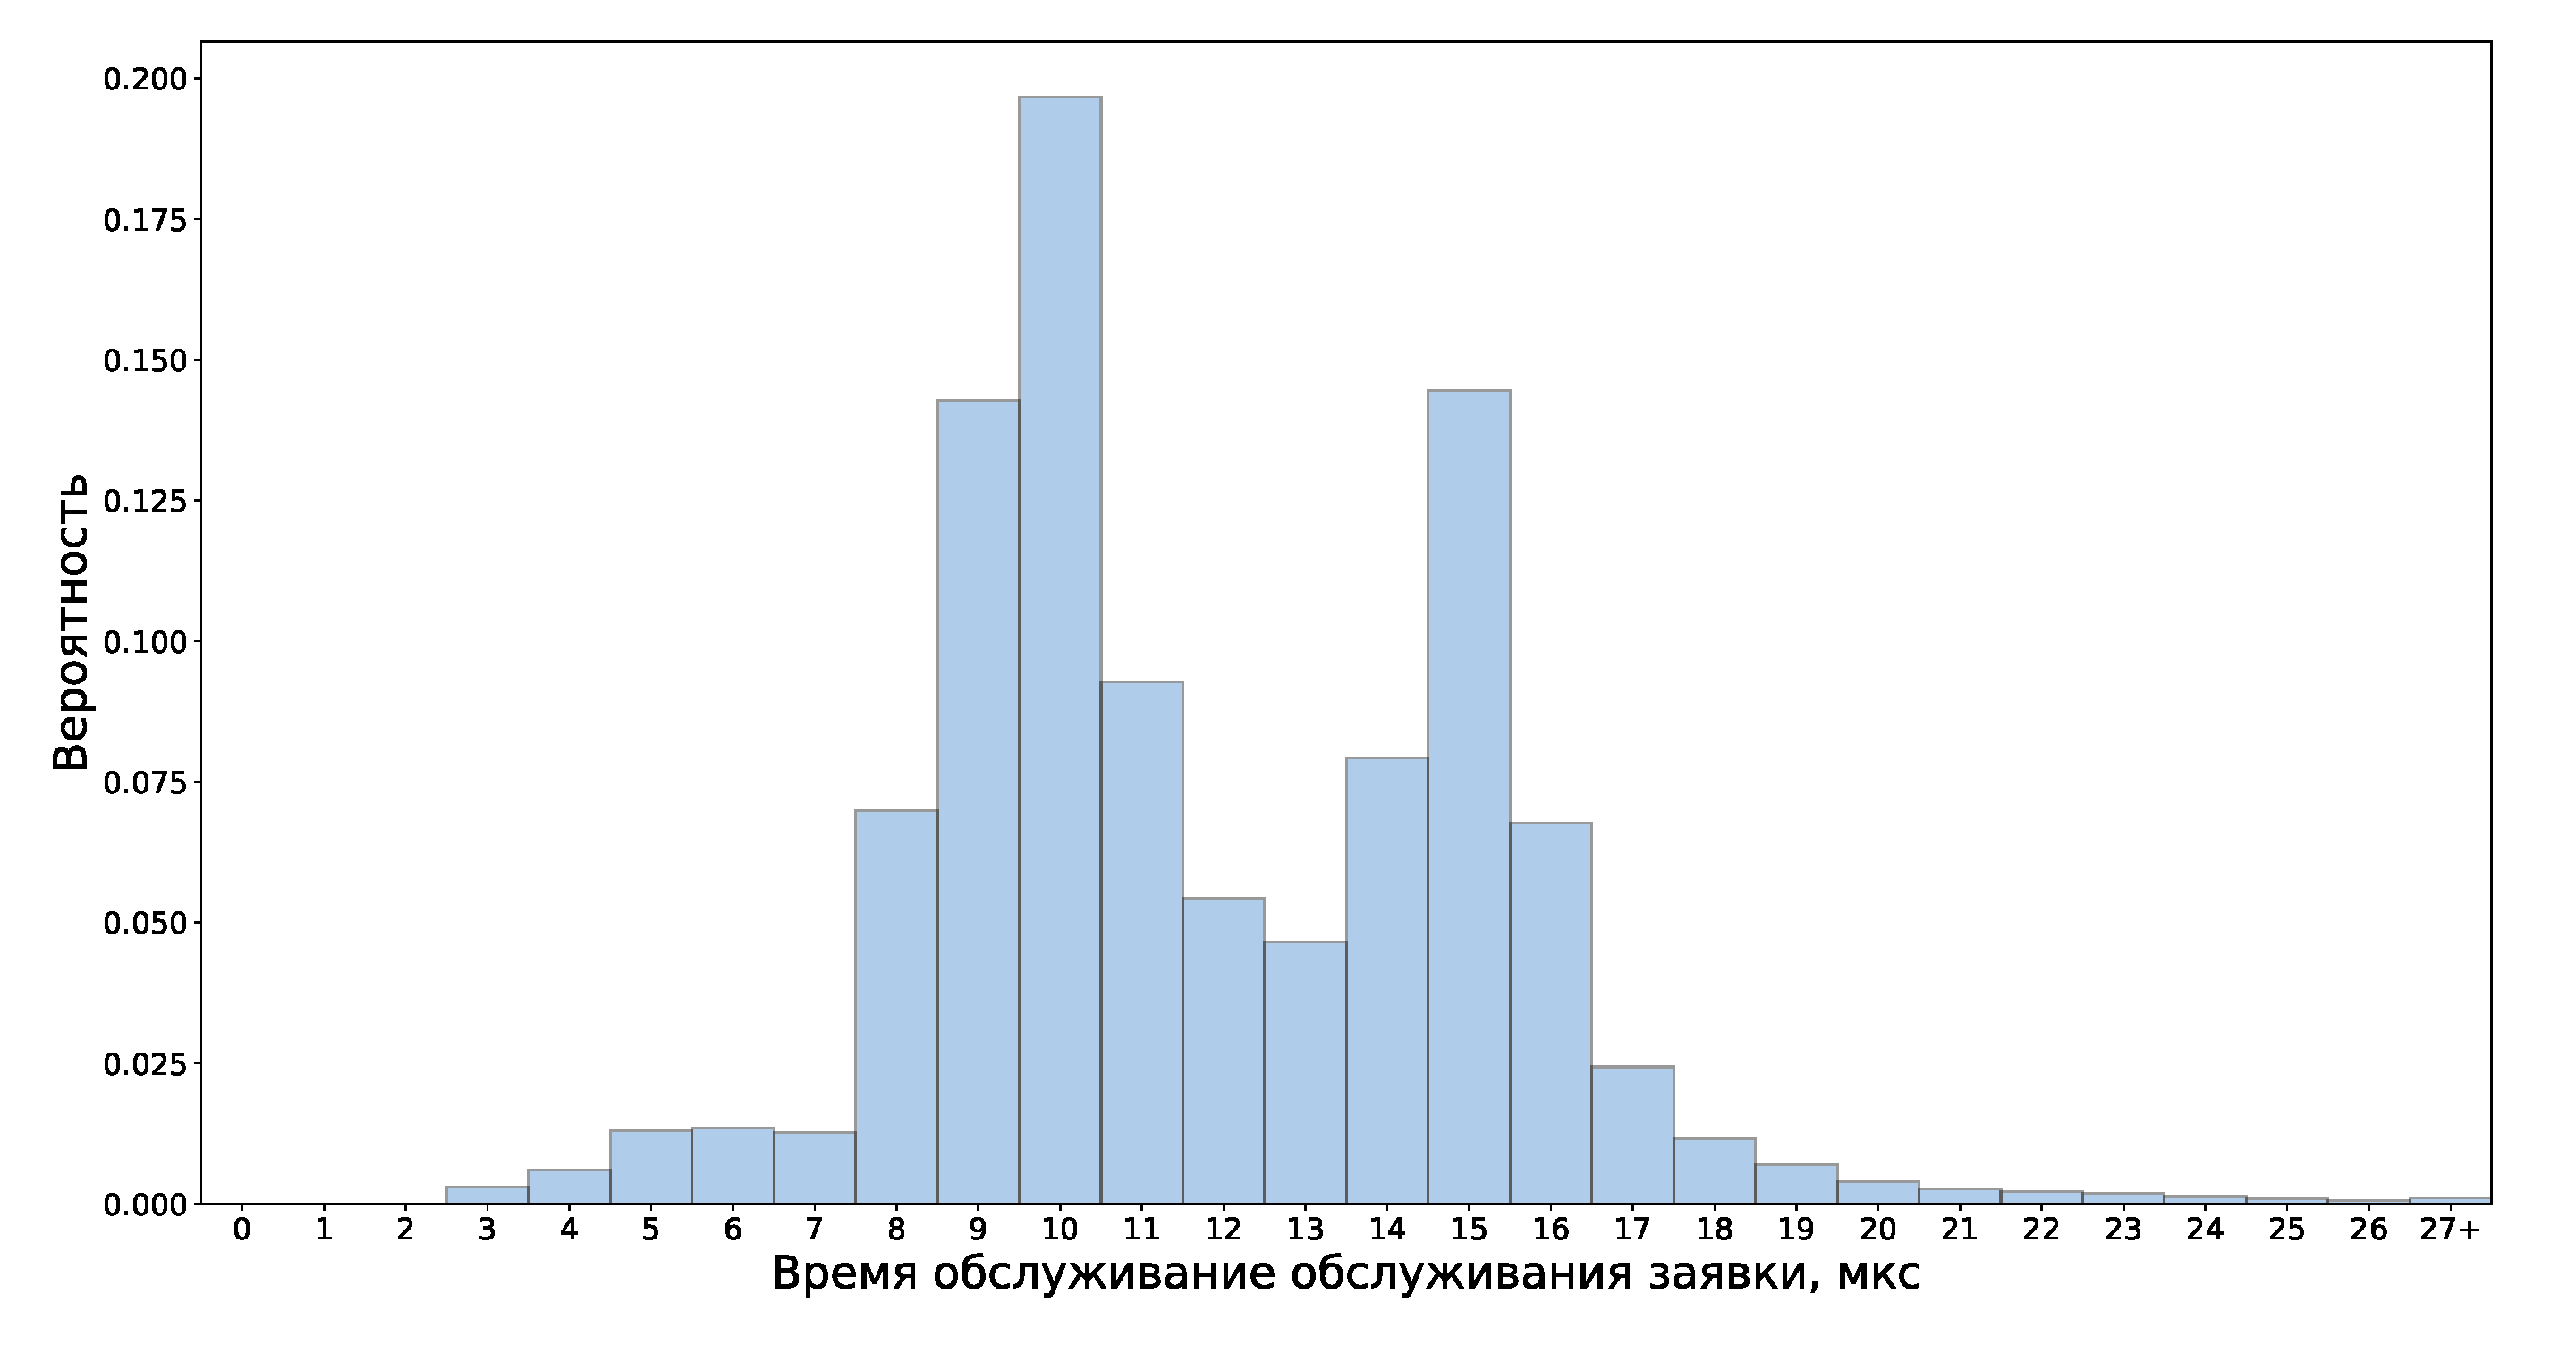
\includegraphics[width=\textwidth]{../../graphics/hist/Engine}
\end{figure}

На Рисунке \ref{chapter41:TRLatency} представлена гистограмма времени обслуживания заявок в процессе-шлюзе. Время обслуживания заявок с 95\% доверительной вероятностью укладывается в диапазон \textit{18.5 $\pm$ 5.5 мкс}.
\begin{figure}[!h]
\caption{Гистограмма времени обслуживания заявки в процессе-шлюзе}
\label{chapter41:TRLatency}
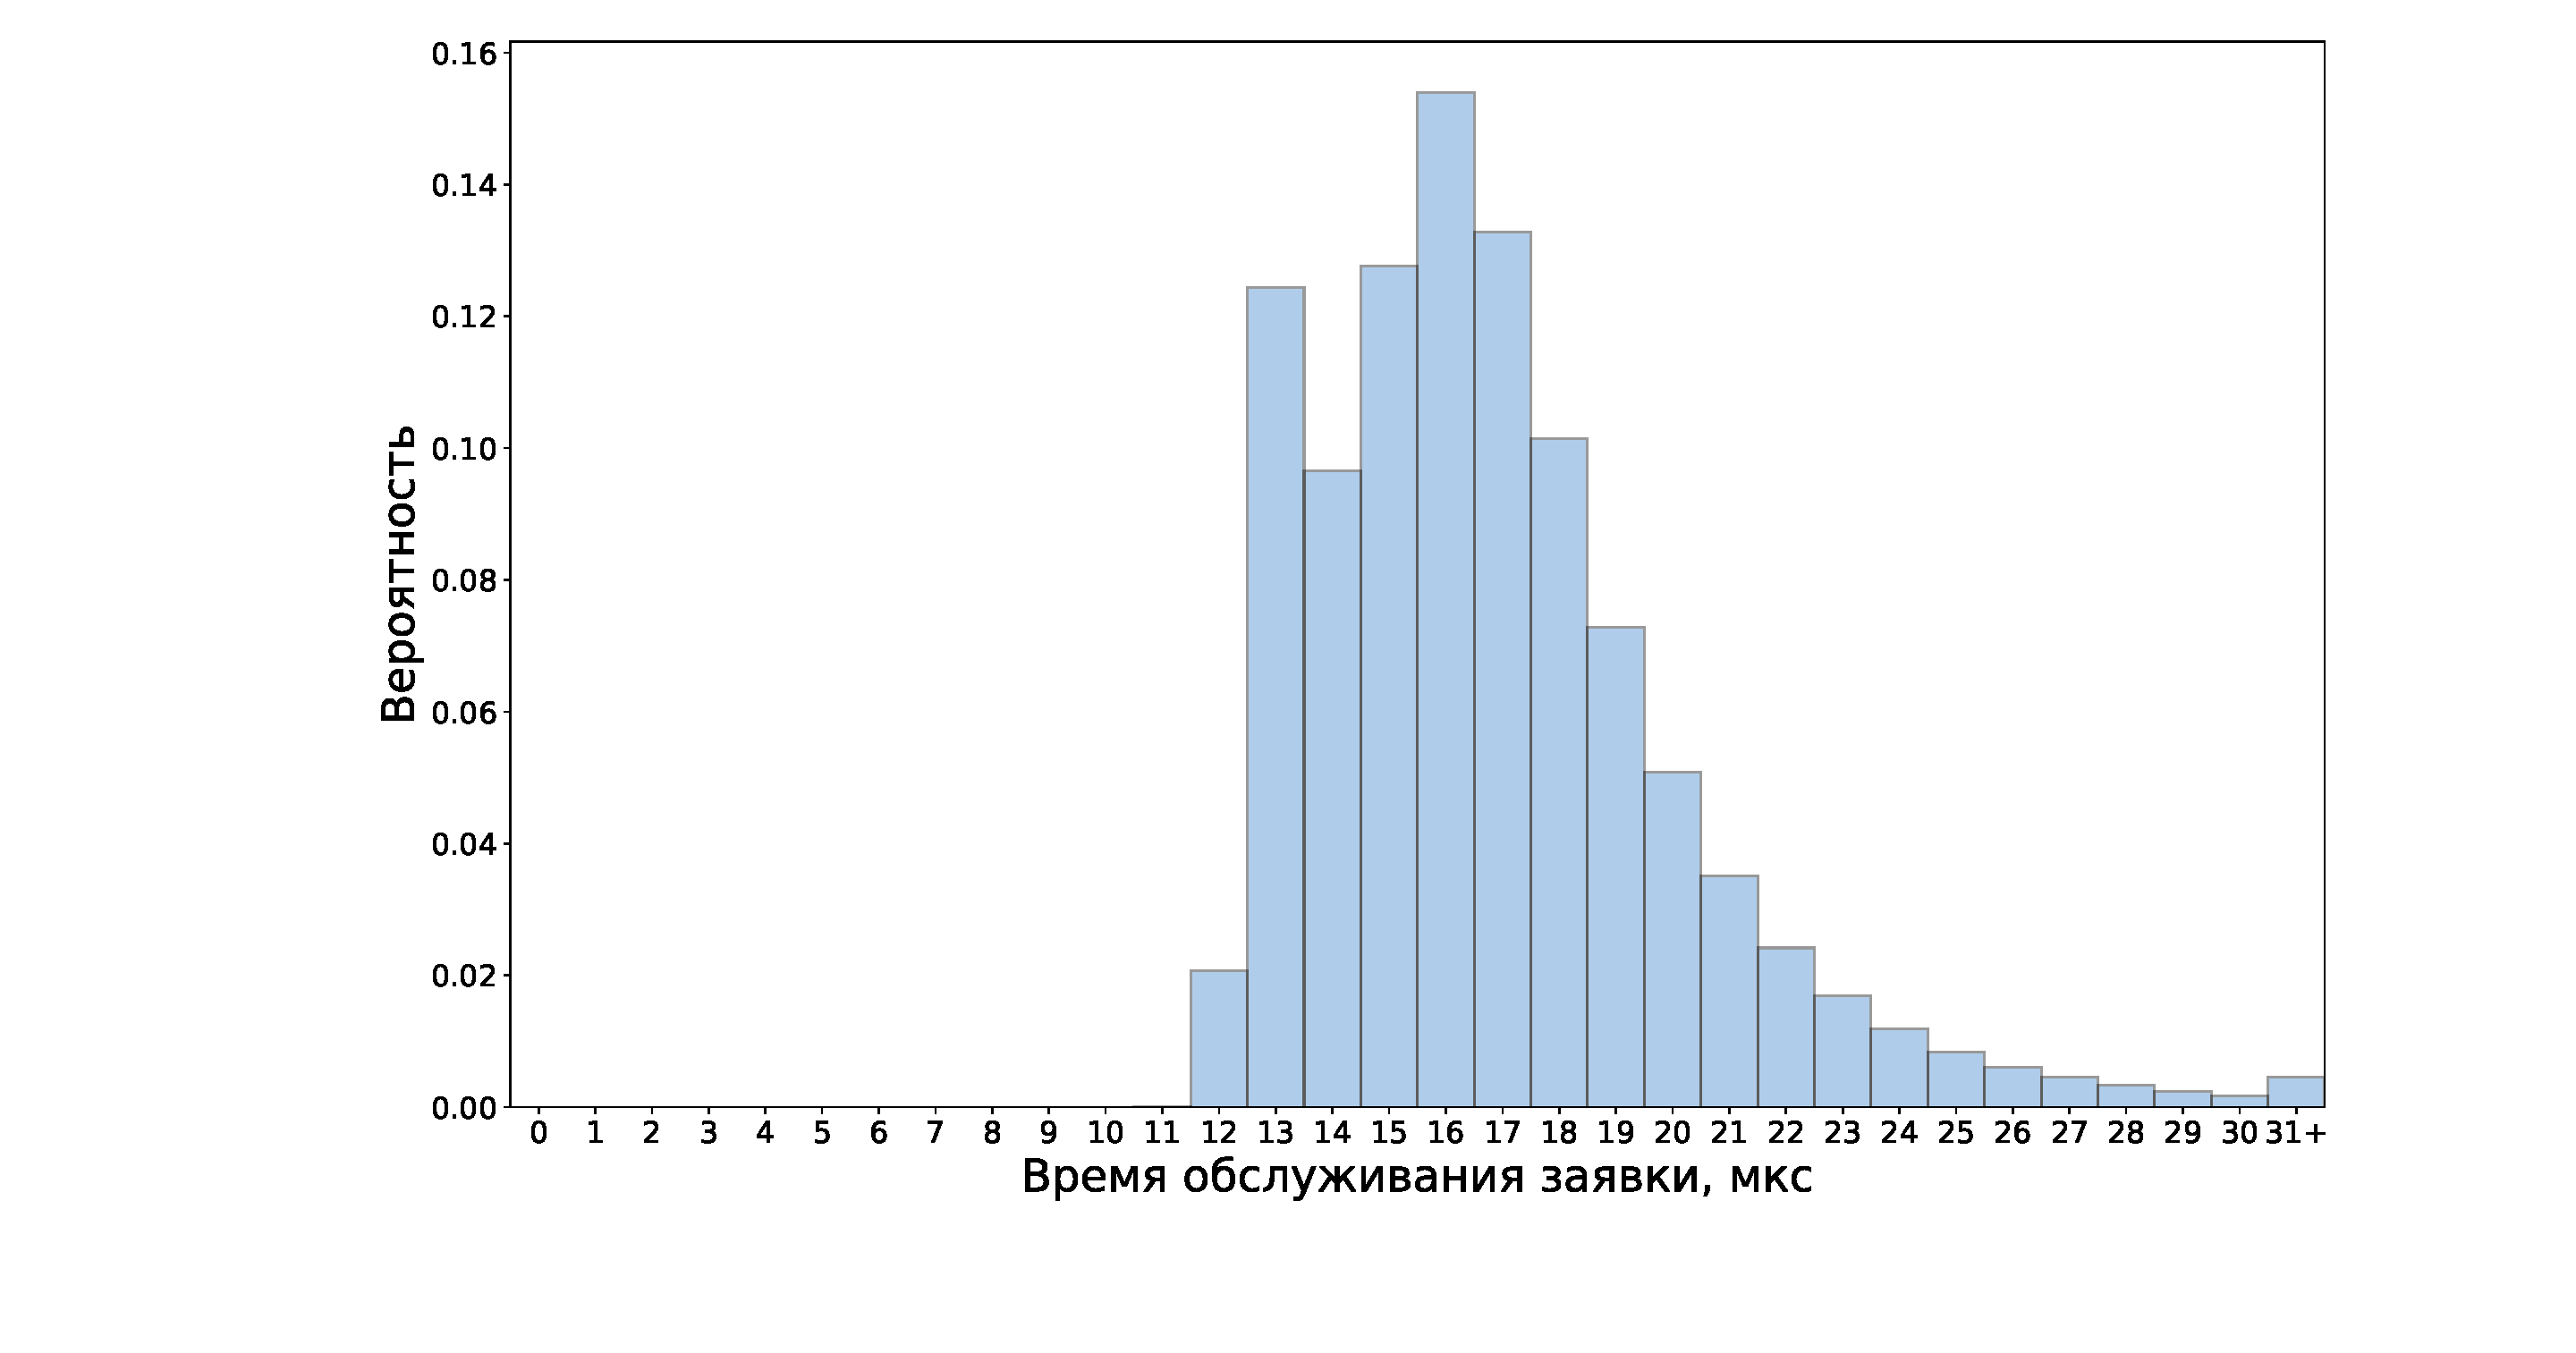
\includegraphics[width=\textwidth]{../../graphics/hist/TR}
\end{figure}


\section{Результаты экспериментов}

\subsection{Использование TCP для передачи данных}

В качестве точки отсчета в настоящей работе выступает метод межпроцессного взаимодействия на основе TCP, используемый посредством сокетов \textbf{TBD: ссылка на определение и на раздел диссертации} \ref{chapter31:PureTCP}. Гистограмма временной задержки на передачу данных для данного метода приведена на Рисунке \ref{chapter41:FigPureTCP}.

\begin{figure}[!h]
\caption{Гистограмма временной задержки на передачу данных между процессами при использовании TCP}
\label{chapter41:FigPureTCP}
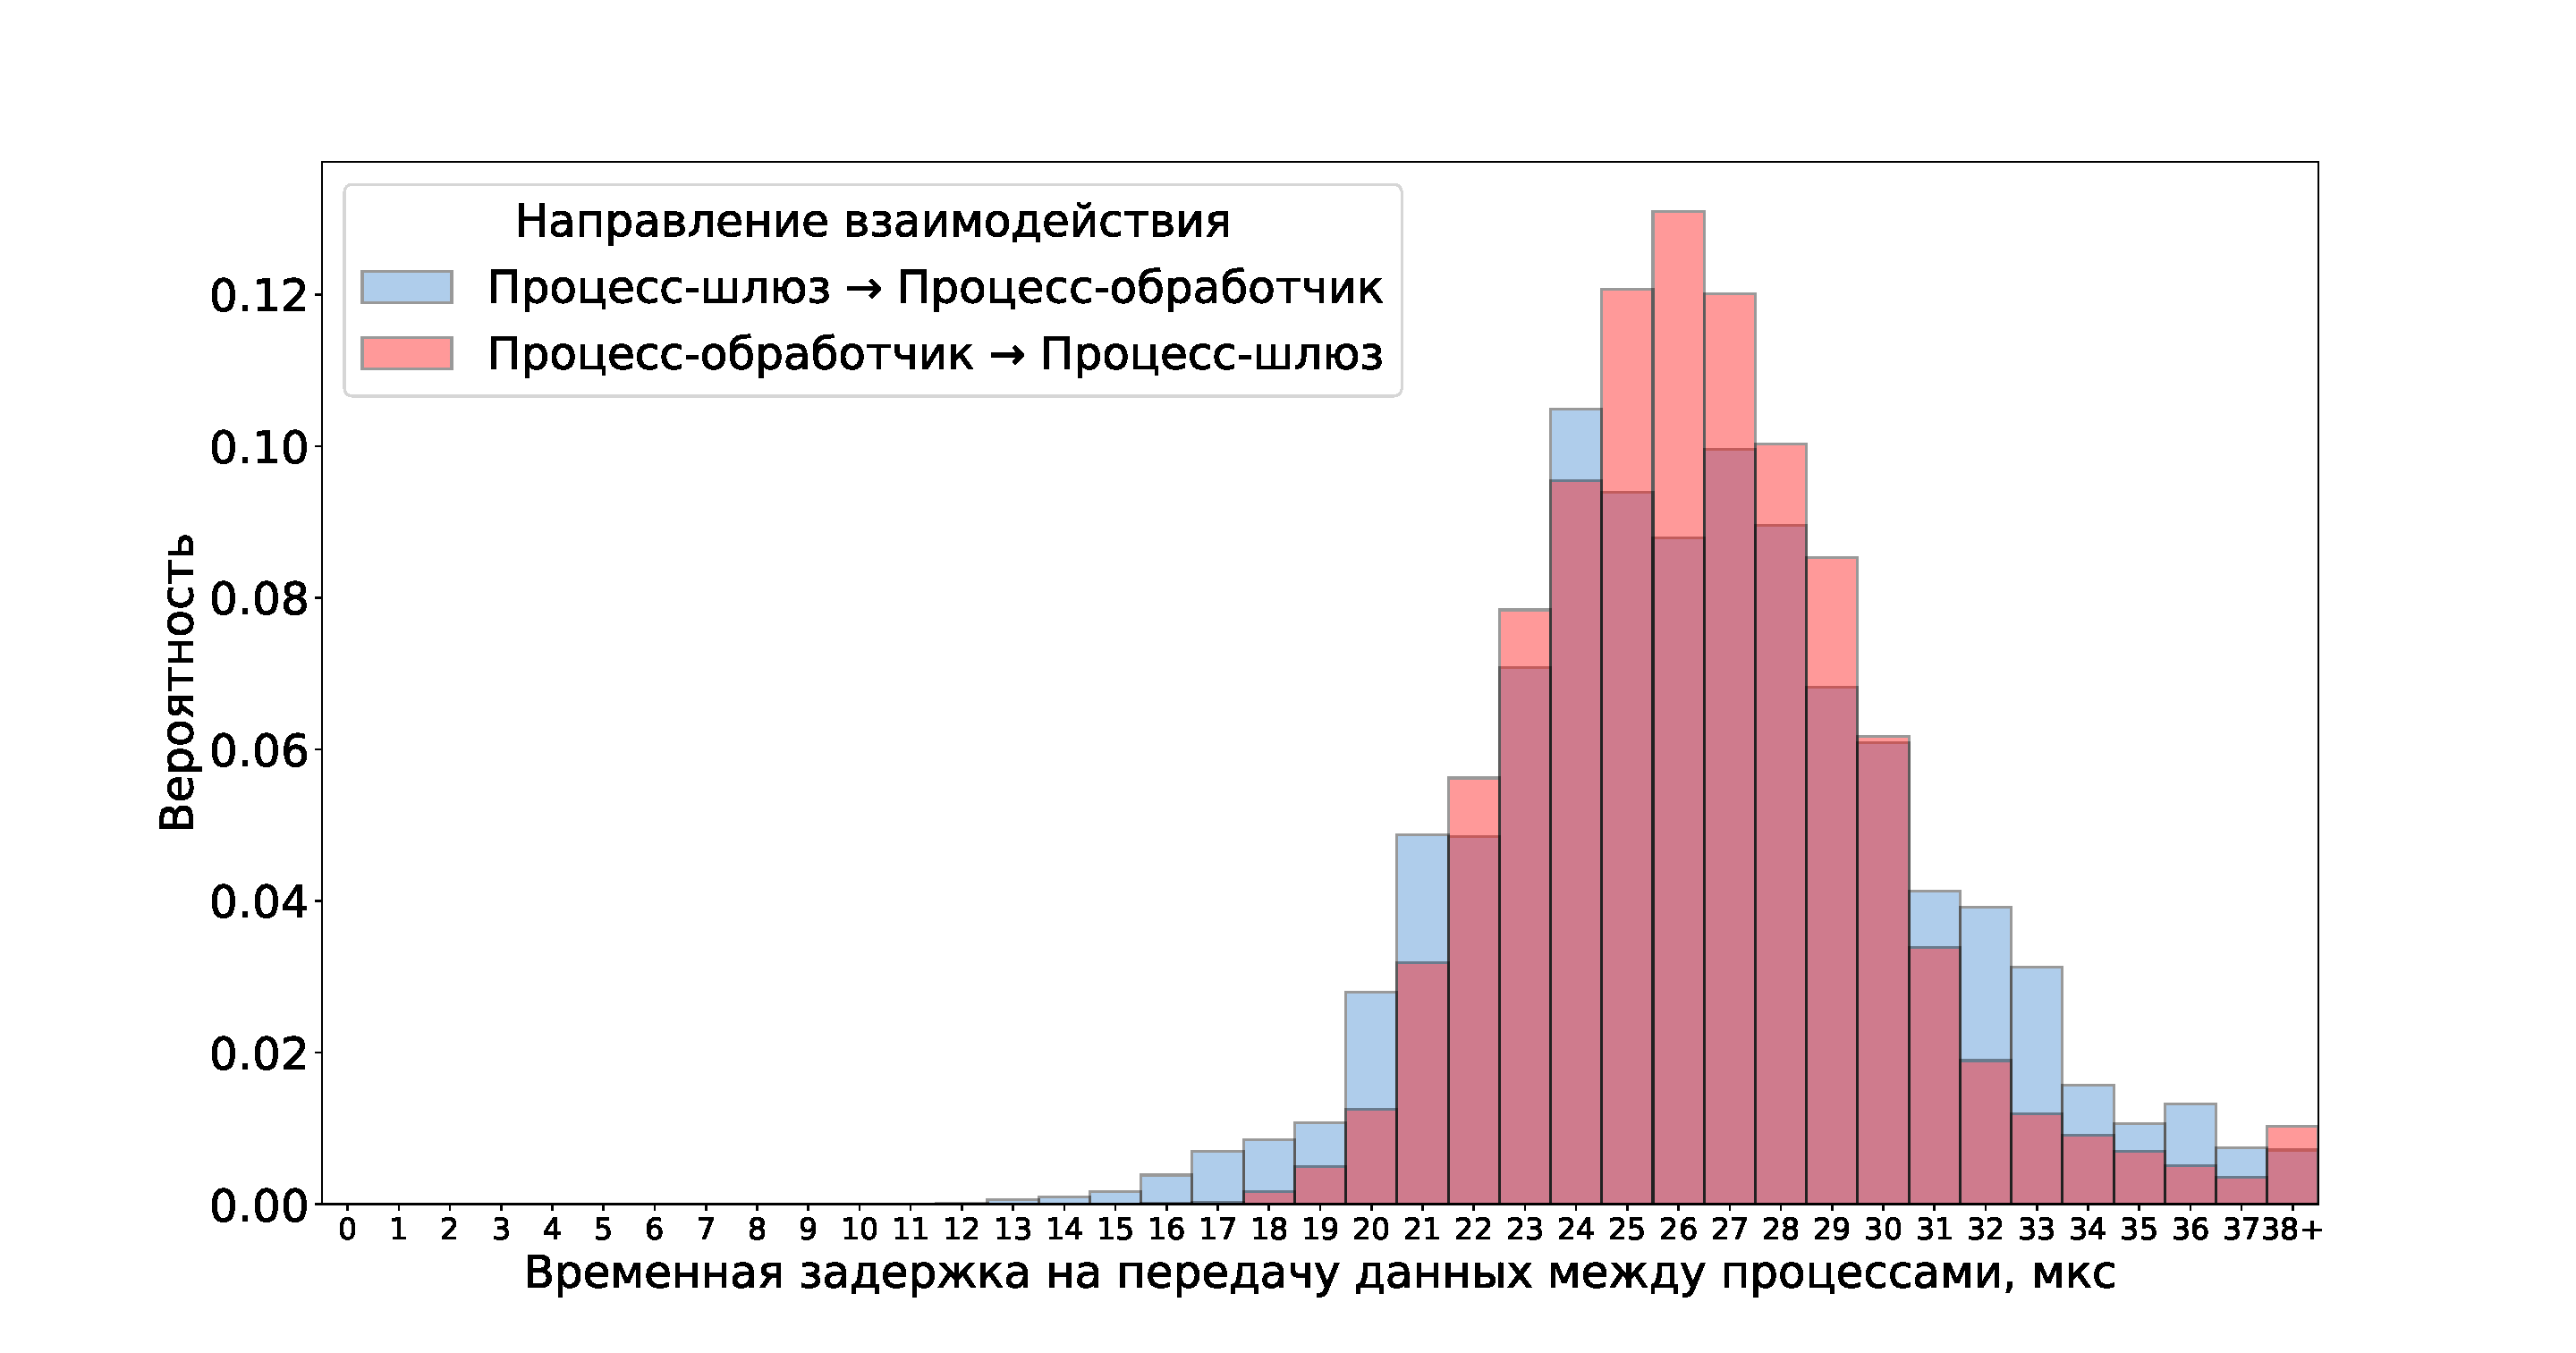
\includegraphics[width=\textwidth]{../../graphics/hist/PureTCP}
\end{figure}

В Таблице \ref{chapter41:TablePureTCP} приведены основные временные характеристики данного метода. Межпроцессное взаимодействие в обе стороны имеет похожие значения.

\begin{table}[!h]
\caption{Основные показатели временной задержки на передачу данных для метода на основе TCP}\label{chapter41:TablePureTCP}
\centering
\resizebox{\textwidth}{!}{
\begin{tabular}{|l|c|c|c|c|c|}
\hline
\begin{tabular}[c]{@{}l@{}}Направление\\ взаимодействия\end{tabular} & \multicolumn{1}{l|}{min(t), мкс} & \multicolumn{1}{l|}{\begin{tabular}[c]{@{}l@{}}M(t) $\pm$ 95\%,\\ мкс\end{tabular}} & \multicolumn{1}{l|}{max(t), мс} & \multicolumn{1}{l|}{\begin{tabular}[c]{@{}l@{}}$\delta$ между\\ сериями, мс\end{tabular}} & \multicolumn{1}{l|}{\begin{tabular}[c]{@{}l@{}}$\delta$ между\\ заявками, мкс\end{tabular}} \\ \hline
\begin{tabular}[c]{@{}l@{}}Процесс-шлюз\\ $\rightarrow$\\ Процесс-обработчик\end{tabular} & 9 & 27.5 $\pm$ 8.5 & 2.1 & 10 $\pm$ 4 & 50 $\pm$ 26 \\ \hline
\begin{tabular}[c]{@{}l@{}}Процесс-обработчик\\ $\rightarrow$\\ Процесс-шлюз\end{tabular} & 13 & 28 $\pm$ 7 & 9.2 & 10 $\pm$ 4 & 87 $\pm$ 32 \\ \hline
\end{tabular}
}
\end{table}

\subsection{Использование разделяемой памяти для передачи данных}

\subsubsection{Использование TCP для оповещения о появлении данных}

В данном подразделе приведены данные об экспериментах с методом межпроцессного взаимодействия, описанным в Разделе \ref{chapter31:SignalTCP}.

\begin{figure}[!h]
\caption{Гистограмма временной задержки на передачу данных между процессами при использовании разделяемой памяти для передачи данных и TCP для оповещения о появлении данных в ней}
\label{chapter41:FigSignalTCP}
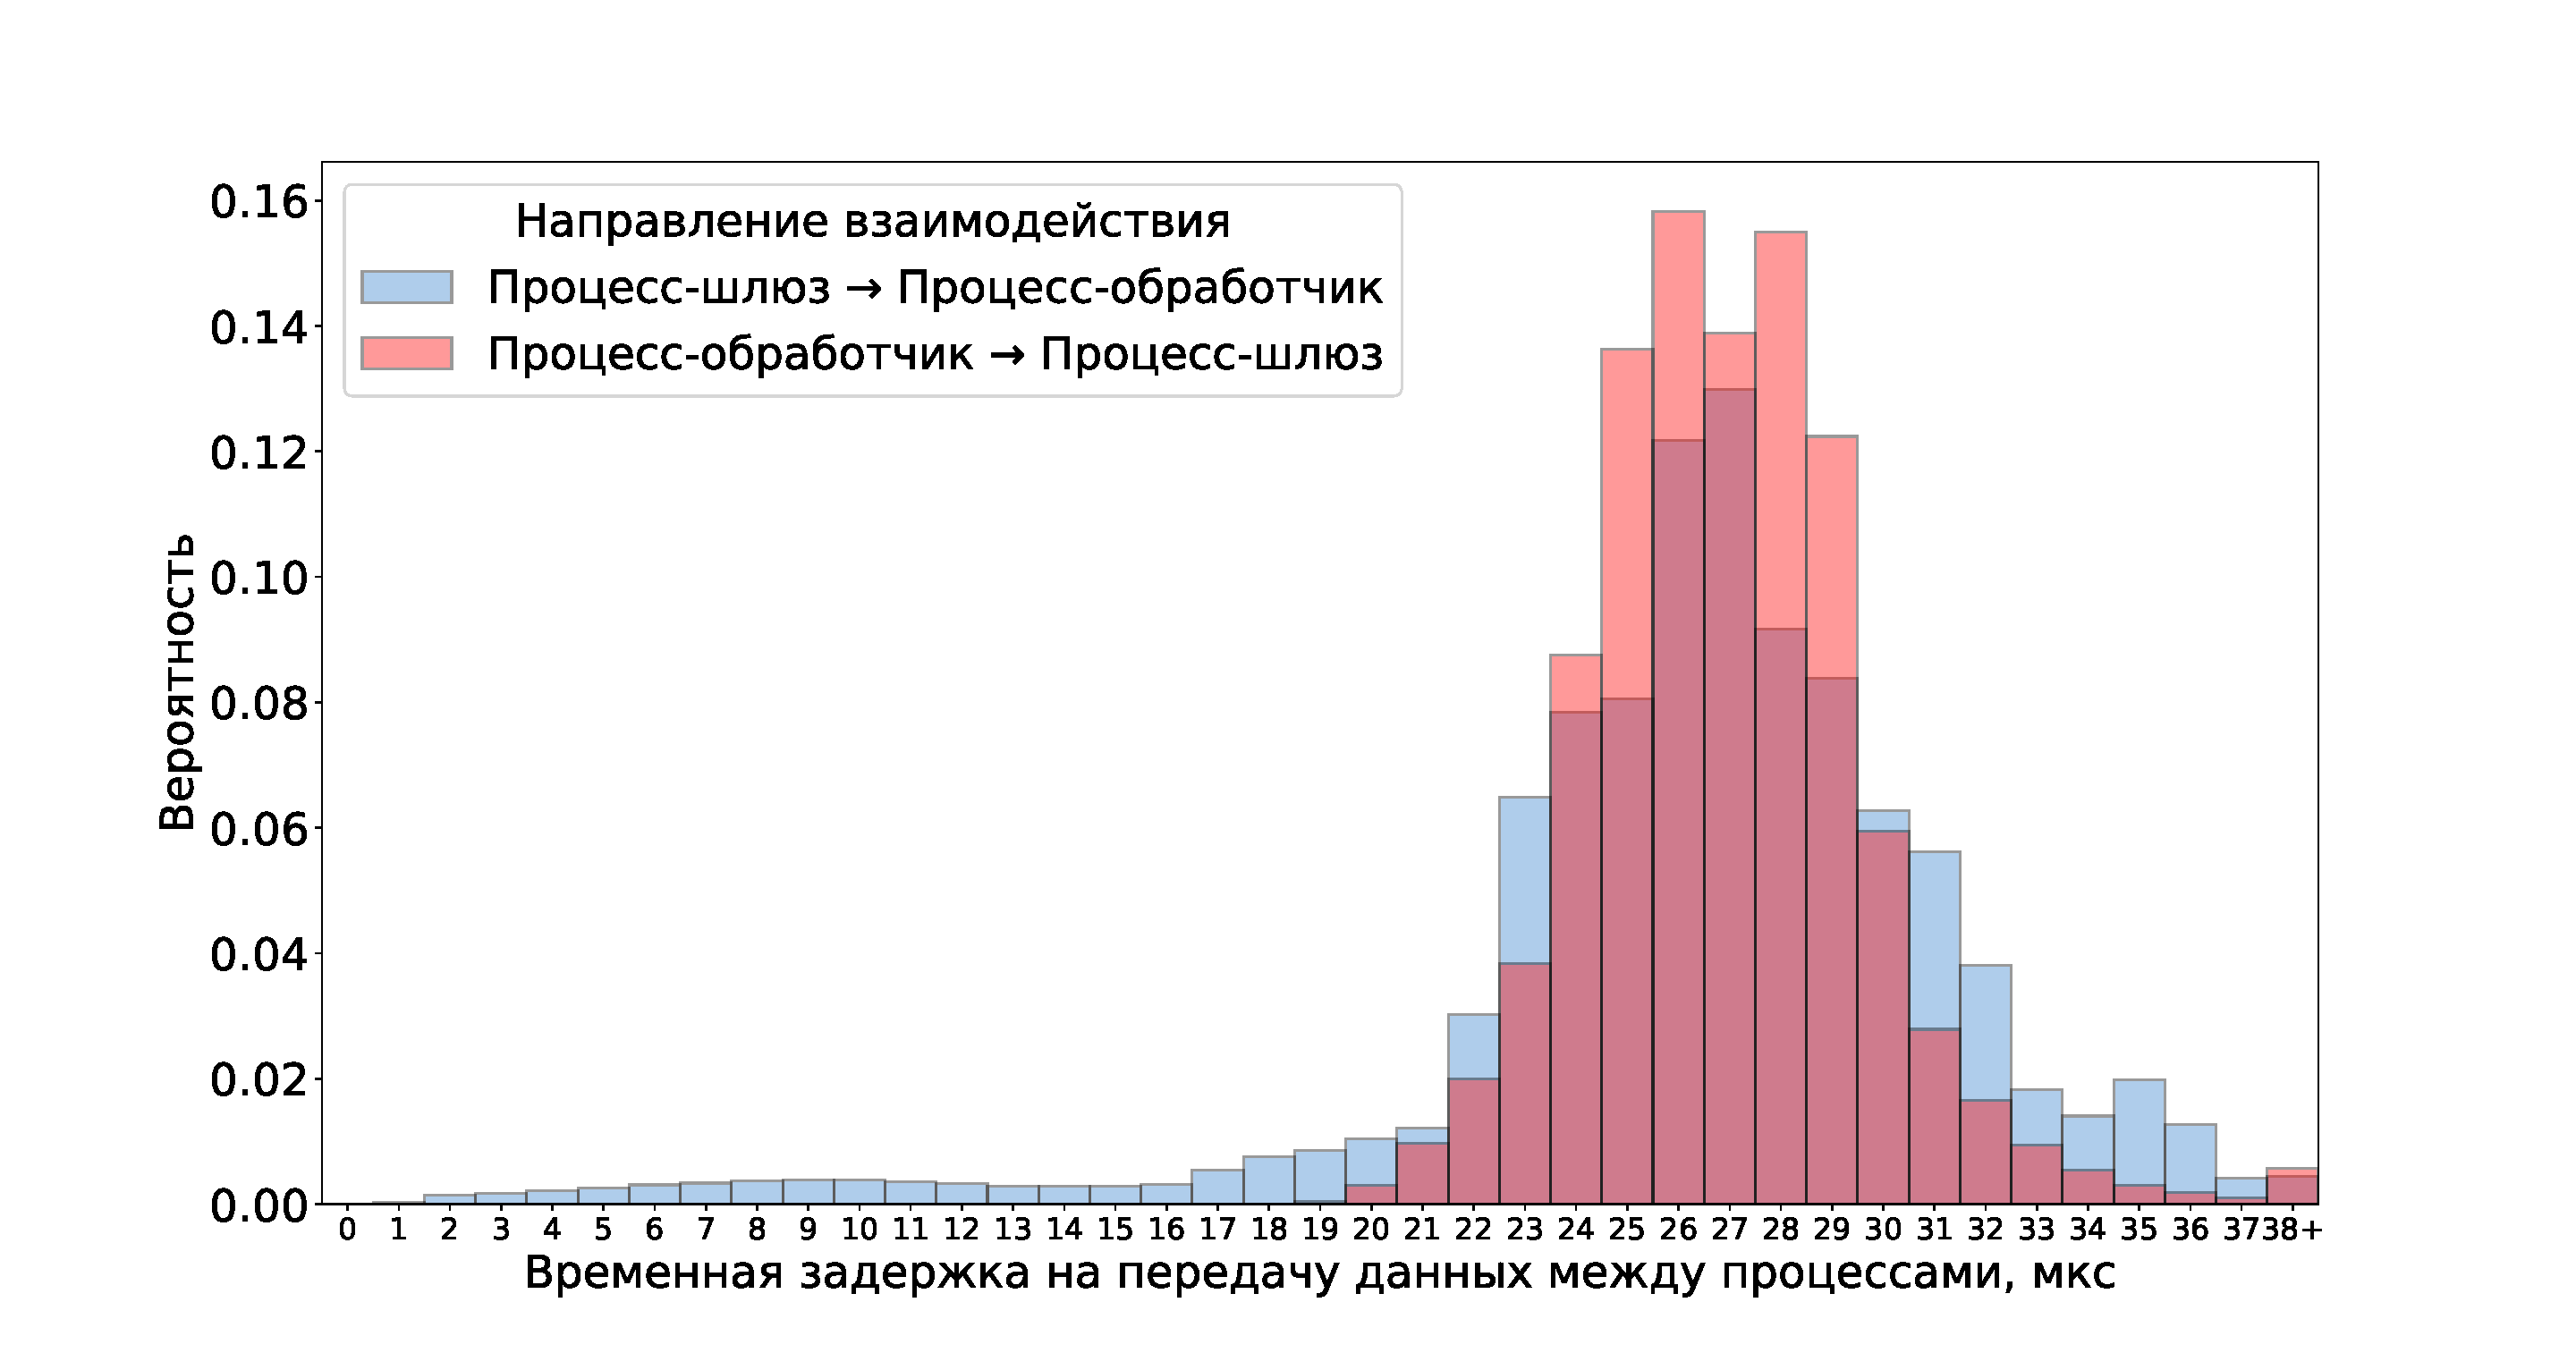
\includegraphics[width=\textwidth]{../../graphics/hist/SignalTCP}
\end{figure}

В Таблице \ref{chapter41:TableSignalTCP} приведены основные временные характеристики данного метода. Межпроцессное взаимодействие в сторону процесса-обработчика работает быстрее, т.к. в среднем время обслуживания заявок в процессе-обработчике заметно меньше (см. Рисунок \ref{chapter41:EngineLatency}), чем скорость поступления новых заявок, что позволяет использовать оптимизацию, описанную в Разделе \ref{chapter31:SharedMemoryOptimization} \textbf{TBD: сослаться на оптимизацию про отсутствие необходимости отправки новых сигналов, когда старые еще не были обработаны.}.

\begin{table}[!h]
\caption{Основные показатели временной задержки на передачу данных для метода на основе TCP}\label{chapter41:TableSignalTCP}
\centering
\resizebox{\textwidth}{!}{
\begin{tabular}{|l|c|c|c|c|c|}
\hline
\begin{tabular}[c]{@{}l@{}}Направление\\ взаимодействия\end{tabular} & \multicolumn{1}{l|}{min(t), мкс} & \multicolumn{1}{l|}{\begin{tabular}[c]{@{}l@{}}M(t) $\pm$ 95\%,\\ мкс\end{tabular}} & \multicolumn{1}{l|}{max(t), мс} & \multicolumn{1}{l|}{\begin{tabular}[c]{@{}l@{}}$\delta$ между\\ сериями, мс\end{tabular}} & \multicolumn{1}{l|}{\begin{tabular}[c]{@{}l@{}}$\delta$ между\\ заявками, мкс\end{tabular}} \\ \hline
\begin{tabular}[c]{@{}l@{}}Процесс-шлюз\\ $\rightarrow$\\ Процесс-обработчик\end{tabular} & 1 & 22.5 $\pm$ 12.5 & 3 & 10 $\pm$ 4 & 50 $\pm$ 27 \\ \hline
\begin{tabular}[c]{@{}l@{}}Процесс-обработчик\\ $\rightarrow$\\ Процесс-шлюз\end{tabular} & 2 & 27.5 $\pm$ 5.5 & 9.8 & 10 $\pm$ 4 & 87 $\pm$ 32 \\ \hline
\end{tabular}
}
\end{table}

\subsubsection{Использование мультиплексора в разделяемой памяти для оповещения о появлении данных}

В данном подразделе приведены данные об экспериментах с методом межпроцессного взаимодействия, описанным в Разделе \ref{chapter31:SignalTCP}.

\paragraph{Блокирующие методы}

В блокирующих методах поток мультиплексора событий использует примитив \textit{futex} \textbf{Может, сослаться на определение futex?} для пассивного ожидания новых сигналов (см. Раздел \ref{chapter31:BlockingMux}).

\subparagraph{Диспетчеризация и обработка соединений по модели "Полусинхронный/Полуреактивный"}

В данном подразделе приведены данные об экспериментах с методом межпроцессного взаимодействия, описанным в Разделе \ref{chapter31:BlockingHSHA}.

В Таблице \ref{chapter41:TableBlockingHSHA} приведены основные временные характеристики данного метода. \textbf{TBD}

На Рисунке \ref{chapter41:FigBlockingHSHA} приведена плотность вероятности временной задержки на передачу данных для данного метода.

\begin{figure}[!h]
\caption{Гистограмма временной задержки на передачу данных между процессами для метода, использующего разделяемую память для передачи данных, блокирующий мультиплексор в разделяемой памяти и модель ''Полусинхронный/Полуреактивный`` при обслуживании заявок}
\label{chapter41:FigBlockingHSHA}
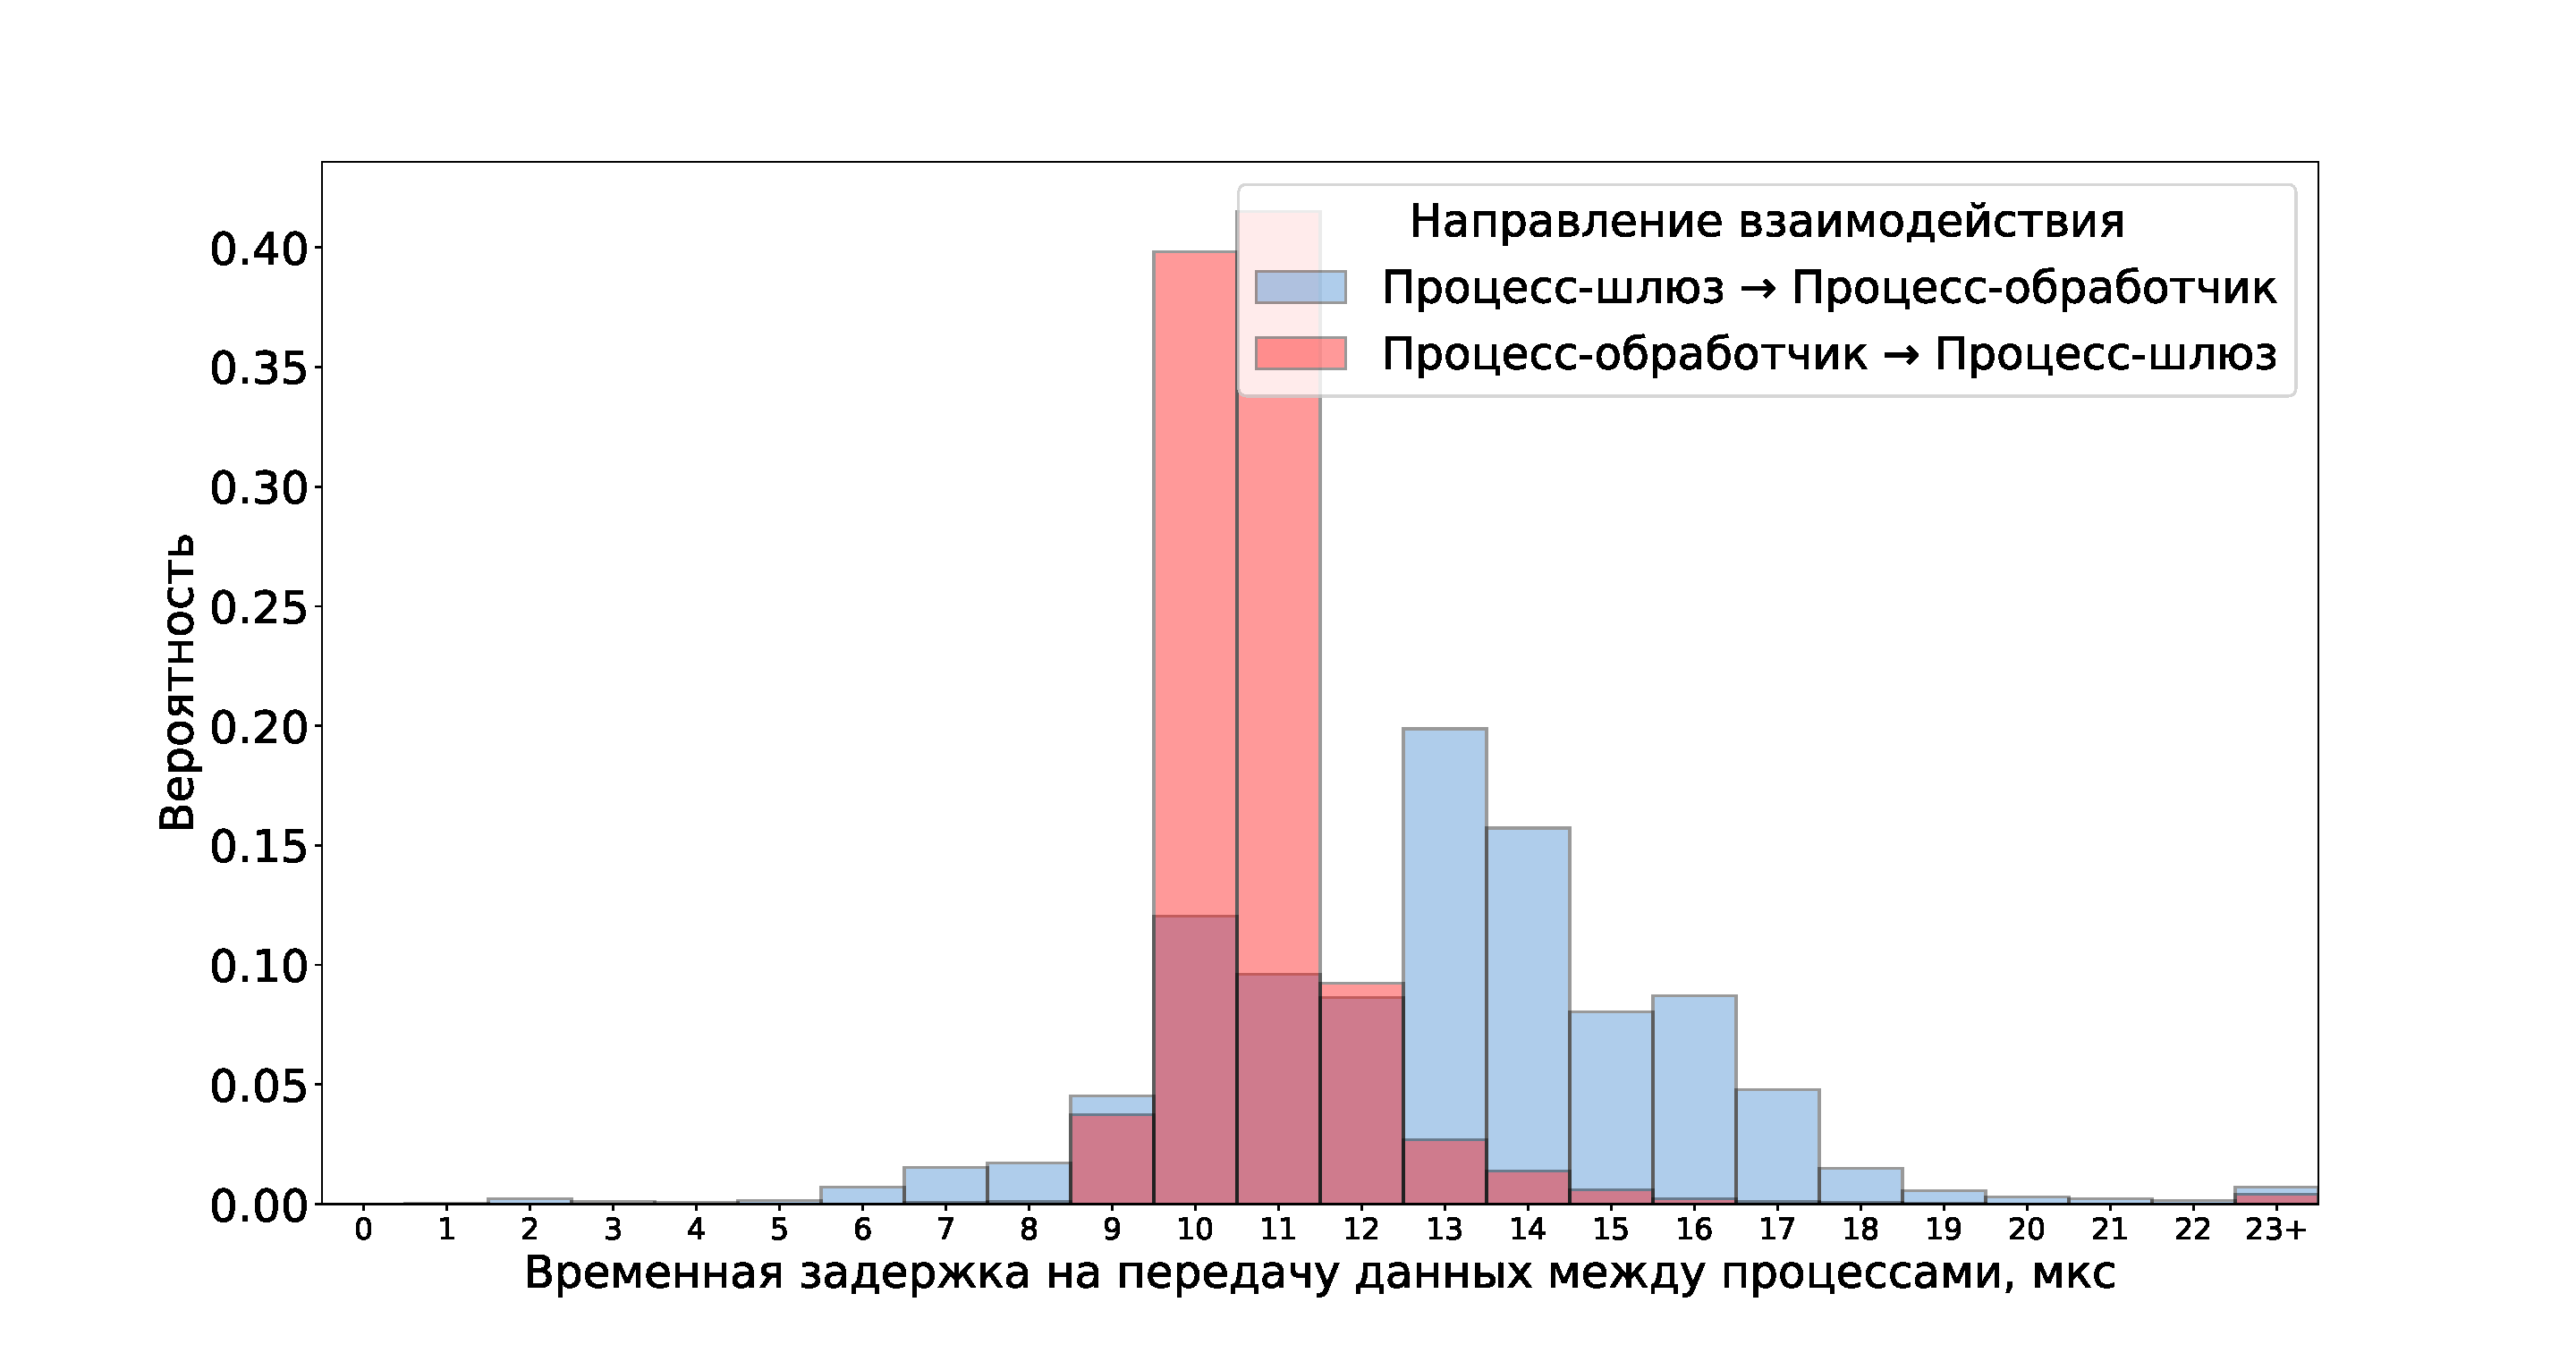
\includegraphics[width=\textwidth]{../../graphics/hist/BlockingHSHA}
\end{figure}
%
%В Таблице \ref{chapter41:TableBlockingHSHA} приведены основные временные характеристики данного метода. Межпроцессное взаимодействие в сторону процесса-обработчика работает быстрее, т.к. в среднем время обслуживания заявок в процессе-обработчике заметно меньше (см. Рисунок \ref{chapter41:EngineLatency}), чем скорость поступления новых заявок, что позволяет использовать оптимизацию, описанную в Разделе \ref{chapter31:SharedMemoryOptimization} \textbf{TBD: сослаться на оптимизацию про отсутствие необходимости отправки новых сигналов, когда старые еще не были обработаны.}.

\begin{table}[!h]
\caption{Основные показатели временной задержки на передачу данных между процессами для метода, использующего разделяемую память для передачи данных, блокирующий мультиплексор в разделяемой памяти и модель ''Полусинхронный/Полуреактивный`` при обслуживании заявок}\label{chapter41:TableBlockingHSHA}
\centering
\resizebox{\textwidth}{!}{
\begin{tabular}{|l|c|c|c|c|c|}
\hline
\begin{tabular}[c]{@{}l@{}}Направление\\ взаимодействия\end{tabular} & \multicolumn{1}{l|}{min(t), мкс} & \multicolumn{1}{l|}{\begin{tabular}[c]{@{}l@{}}M(t) $\pm$ 95\%,\\ мкс\end{tabular}} & \multicolumn{1}{l|}{max(t), мс} & \multicolumn{1}{l|}{\begin{tabular}[c]{@{}l@{}}$\delta$ между\\ сериями, мс\end{tabular}} & \multicolumn{1}{l|}{\begin{tabular}[c]{@{}l@{}}$\delta$ между\\ заявками, мкс\end{tabular}} \\ \hline
\begin{tabular}[c]{@{}l@{}}Процесс-шлюз\\ $\rightarrow$\\ Процесс-обработчик\end{tabular} & 1 & 12.5 $\pm$ 5.5 & 6.9 & 10 $\pm$ 4 & 51 $\pm$ 28 \\ \hline
\begin{tabular}[c]{@{}l@{}}Процесс-обработчик\\ $\rightarrow$\\ Процесс-шлюз\end{tabular} & 3 & 11.5 $\pm$ 2.5 & 11.6 & 10 $\pm$ 4 & 91 $\pm$ 36 \\ \hline
\end{tabular}
}
\end{table}

\subparagraph{Диспетчеризация и обработка соединений по модели "Лидер/Последователи"}


В данном подразделе приведены данные об экспериментах с методом межпроцессного взаимодействия, описанным в Разделе \ref{chapter31:BlockingLF}.

В Таблице \ref{chapter41:TableBlockingLF} приведены основные временные характеристики данного метода. \textbf{TBD}

На Рисунке \ref{chapter41:FigBlockingLF} приведена плотность вероятности временной задержки на передачу данных для данного метода.

\begin{figure}[!h]
\caption{Гистограмма временной задержки на передачу данных между процессами для метода, использующего разделяемую память для передачи данных, неблокирующий мультиплексор в разделяемой памяти и модель ''Лидер/Последователи`` при обслуживании заявок}
\label{chapter41:FigBlockingLF}
\includegraphics[width=\textwidth]{../../graphics/hist/BlockingLF}
\end{figure}
%
%В Таблице \ref{chapter41:TableBlockingHSHA} приведены основные временные характеристики данного метода. Межпроцессное взаимодействие в сторону процесса-обработчика работает быстрее, т.к. в среднем время обслуживания заявок в процессе-обработчике заметно меньше (см. Рисунок \ref{chapter41:EngineLatency}), чем скорость поступления новых заявок, что позволяет использовать оптимизацию, описанную в Разделе \ref{chapter31:SharedMemoryOptimization} \textbf{TBD: сослаться на оптимизацию про отсутствие необходимости отправки новых сигналов, когда старые еще не были обработаны.}.

\begin{table}[!h]
\caption{Основные показатели временной задержки на передачу данных между процессами для метода, использующего разделяемую память для передачи данных, неблокирующий мультиплексор в разделяемой памяти и модель ''Лидер/Последователи`` при обслуживании заявок}\label{chapter41:TableBlockingLF}
\centering
\resizebox{\textwidth}{!}{
\begin{tabular}{|l|c|c|c|c|c|}
\hline
\begin{tabular}[c]{@{}l@{}}Направление\\ взаимодействия\end{tabular} & \multicolumn{1}{l|}{min(t), мкс} & \multicolumn{1}{l|}{\begin{tabular}[c]{@{}l@{}}M(t) $\pm$ 95\%,\\ мкс\end{tabular}} & \multicolumn{1}{l|}{max(t), мс} & \multicolumn{1}{l|}{\begin{tabular}[c]{@{}l@{}}$\delta$ между\\ сериями, мс\end{tabular}} & \multicolumn{1}{l|}{\begin{tabular}[c]{@{}l@{}}$\delta$ между\\ заявками, мкс\end{tabular}} \\ \hline
\begin{tabular}[c]{@{}l@{}}Процесс-шлюз\\ $\rightarrow$\\ Процесс-обработчик\end{tabular} & 1 & 11.5 $\pm$ 6.5 & 2.4 & 8.4 $\pm$ 5.3 & 52 $\pm$ 29 \\ \hline
\begin{tabular}[c]{@{}l@{}}Процесс-обработчик\\ $\rightarrow$\\ Процесс-шлюз\end{tabular} & 2 & 9.5 $\pm$ 1.5 & 9.5 & 8.4 $\pm$ 5.3 & 90 $\pm$ 35 \\ \hline
\end{tabular}
}
\end{table}

\paragraph{Неблокирующий метод}

В неблокирующем методе поток мультиплексора событий метод активного ожидания новых сигналов (см. Раздел \ref{chapter31:NonBlockingMux}). В данном параграфе рассматривается исключительно модель обслуживания заявок ''Лидер/Последователи`` т.к. в параграфе выше она показала лучшие результаты по сравнению с моделью ''Полусинхронный/Полуреактивный``.

\subparagraph{Диспетчеризация и обработка соединений по модели "Лидер/Последователи"}

В данном подразделе приведены данные об экспериментах с методом межпроцессного взаимодействия, описанным в Разделе \ref{chapter31:NonBlockingLF}.

В Таблице \ref{chapter41:TableNonBlockingLF} приведены основные временные характеристики данного метода. \textbf{TBD}

На Рисунке \ref{chapter41:FigNonBlockingLF} приведена плотность вероятности временной задержки на передачу данных для данного метода.

\begin{figure}[!h]
\caption{Гистограмма временной задержки на передачу данных между процессами для метода, использующего разделяемую память для передачи данных, блокирующий мультиплексор в разделяемой памяти и модель ''Лидер/Последователи`` при обслуживании заявок}
\label{chapter41:FigNonBlockingLF}
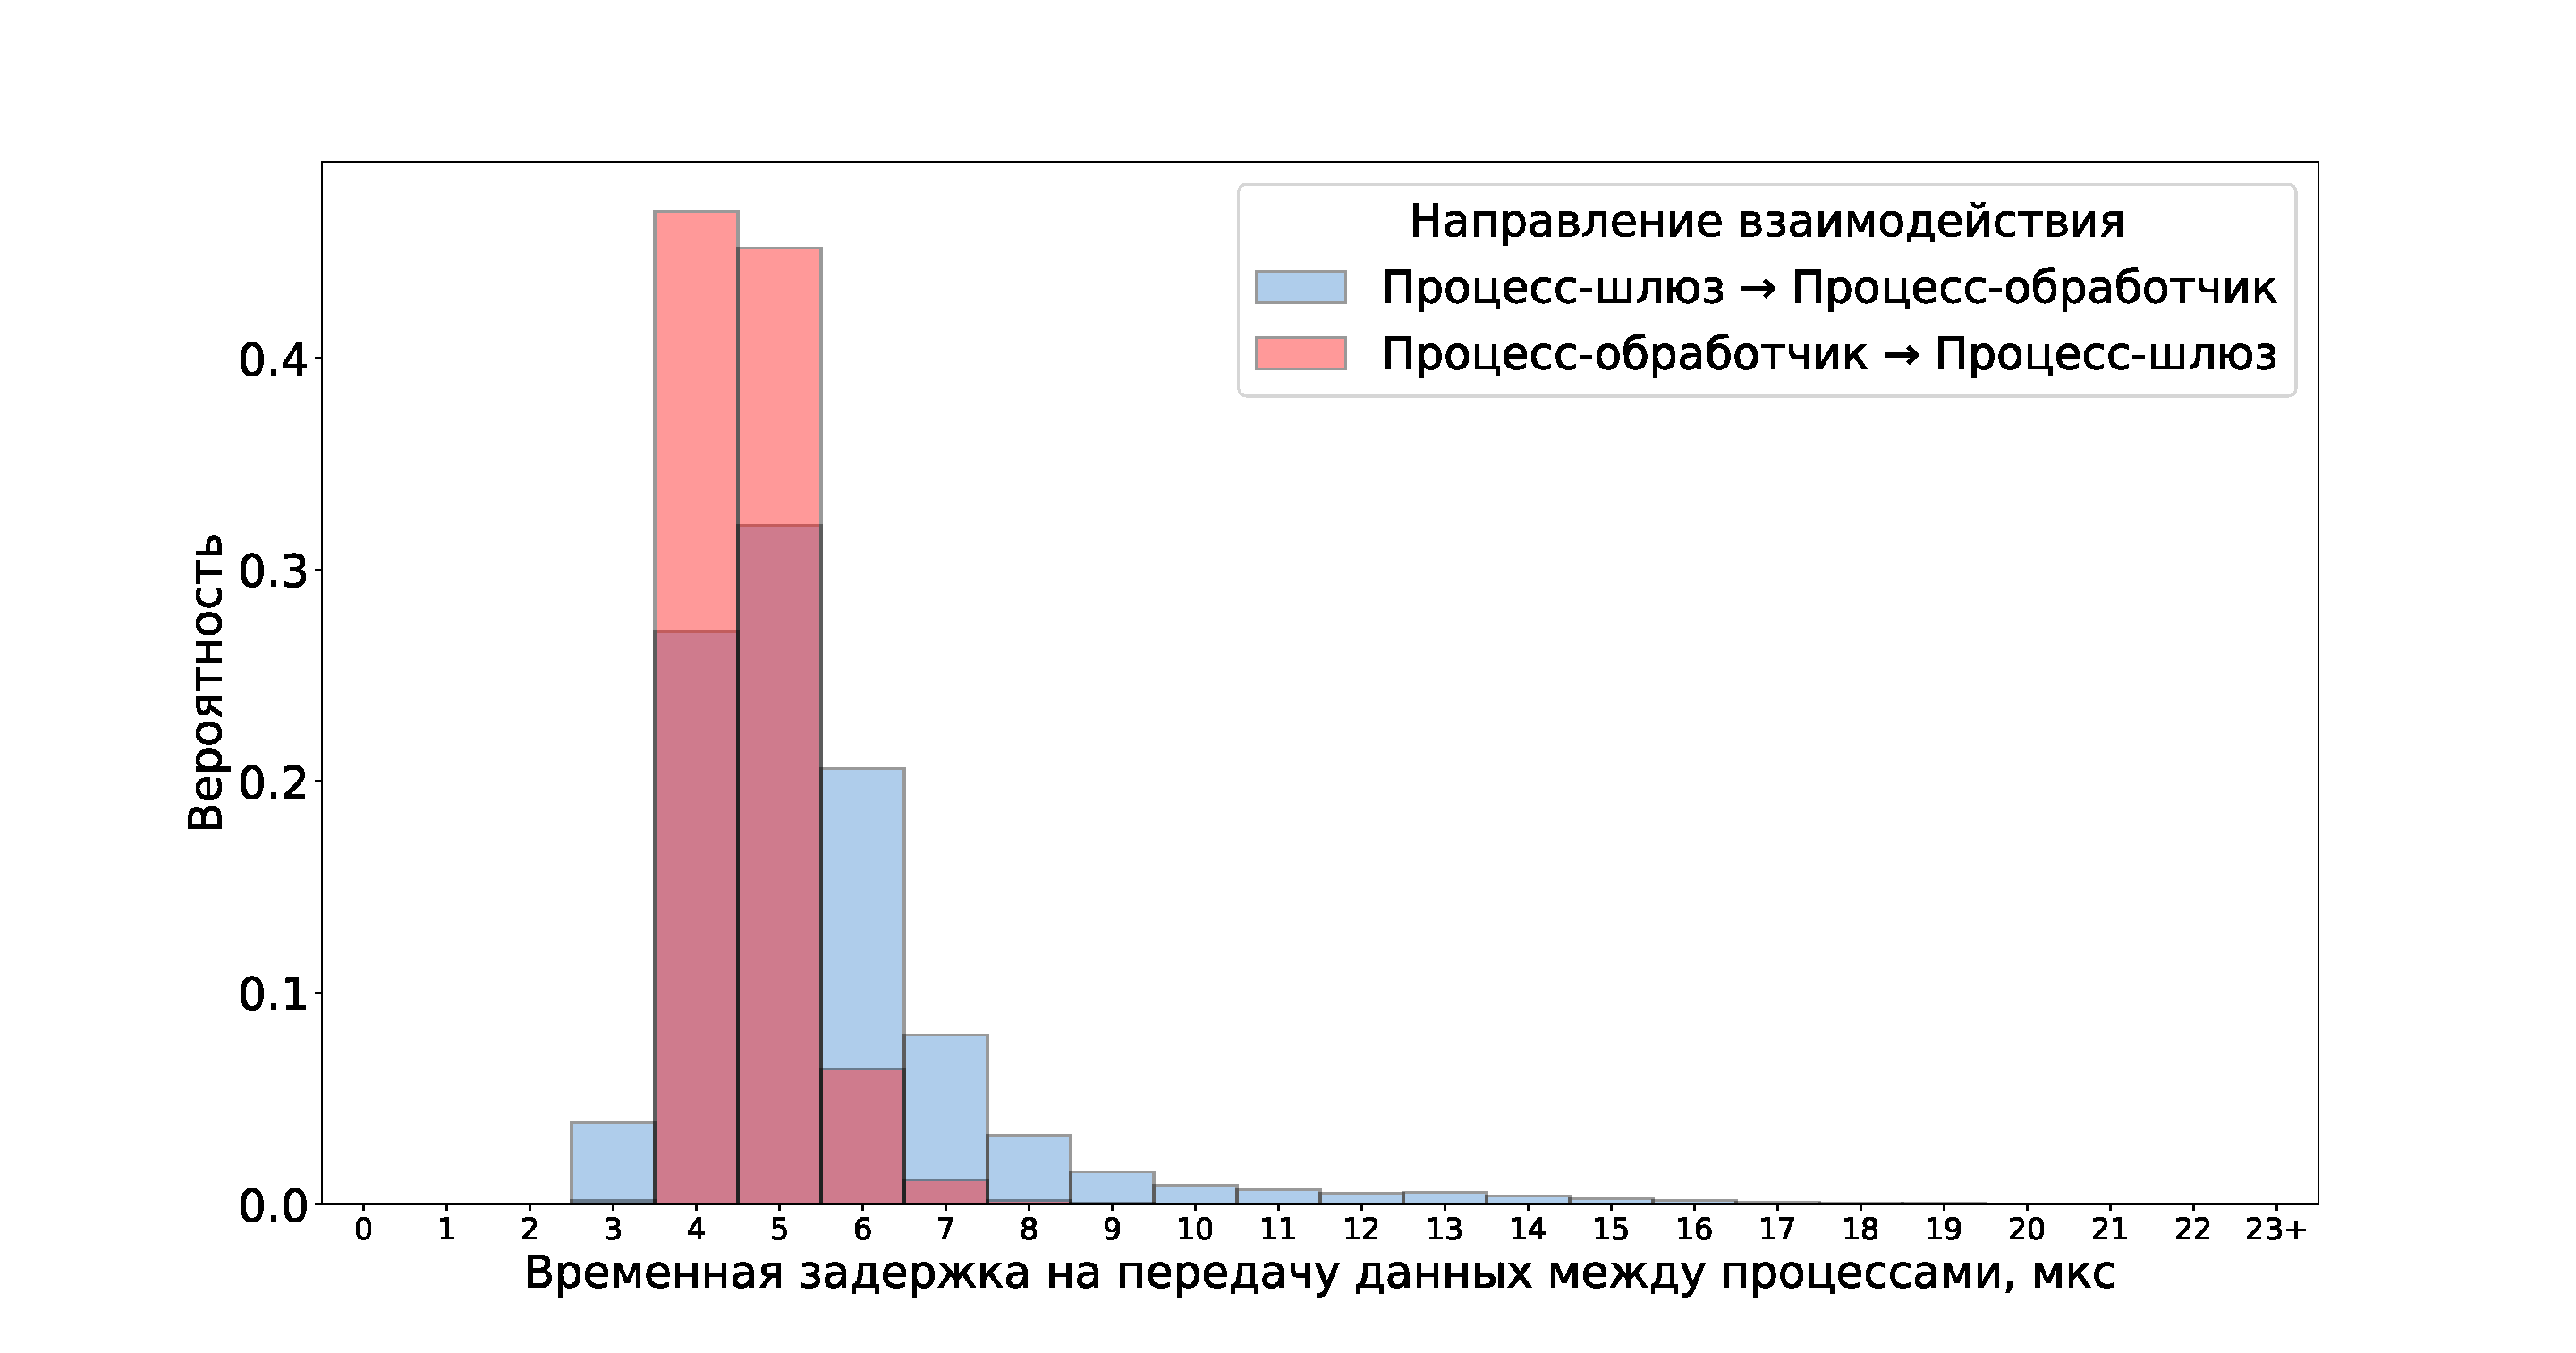
\includegraphics[width=\textwidth]{../../graphics/hist/NonBlockingLF}
\end{figure}
%
%В Таблице \ref{chapter41:TableBlockingHSHA} приведены основные временные характеристики данного метода. Межпроцессное взаимодействие в сторону процесса-обработчика работает быстрее, т.к. в среднем время обслуживания заявок в процессе-обработчике заметно меньше (см. Рисунок \ref{chapter41:EngineLatency}), чем скорость поступления новых заявок, что позволяет использовать оптимизацию, описанную в Разделе \ref{chapter31:SharedMemoryOptimization} \textbf{TBD: сослаться на оптимизацию про отсутствие необходимости отправки новых сигналов, когда старые еще не были обработаны.}.

\begin{table}[!h]
\caption{Основные показатели временной задержки на передачу данных между процессами для метода, использующего разделяемую память для передачи данных, блокирующий мультиплексор в разделяемой памяти и модель ''Лидер/Последователи`` при обслуживании заявок}\label{chapter41:TableNonBlockingLF}
\centering
\resizebox{\textwidth}{!}{
\begin{tabular}{|l|c|c|c|c|c|}
\hline
\begin{tabular}[c]{@{}l@{}}Направление\\ взаимодействия\end{tabular} & \multicolumn{1}{l|}{min(t), мкс} & \multicolumn{1}{l|}{\begin{tabular}[c]{@{}l@{}}M(t) $\pm$ 95\%,\\ мкс\end{tabular}} & \multicolumn{1}{l|}{max(t), мс} & \multicolumn{1}{l|}{\begin{tabular}[c]{@{}l@{}}$\delta$ между\\ сериями, мс\end{tabular}} & \multicolumn{1}{l|}{\begin{tabular}[c]{@{}l@{}}$\delta$ между\\ заявками, мкс\end{tabular}} \\ \hline
\begin{tabular}[c]{@{}l@{}}Процесс-шлюз\\ $\rightarrow$\\ Процесс-обработчик\end{tabular} & 1 & 7 $\pm$ 4 & 8.5 & 7.4 $\pm$ 5.8 & 58 $\pm$ 35 \\ \hline
\begin{tabular}[c]{@{}l@{}}Процесс-обработчик\\ $\rightarrow$\\ Процесс-шлюз\end{tabular} & 3 & 5 $\pm$ 1 & 0.03 & 7.4 $\pm$ 5.8 & 167 $\pm$ 113 \\ \hline
\end{tabular}
}
\end{table}

\chapterconclusion

Вывод по очередной главе